\documentclass{article}
\usepackage{amssymb}
\usepackage{changepage}
\usepackage[fleqn]{amsmath}
\usepackage{gensymb}
\usepackage{cancel}
\usepackage{tkz-euclide}
\usepackage{graphicx}
\title{Pith Ball Lab}
\author{SPH-4UI - Tristan Simpson}

\begin{document}
\maketitle

\vspace{0.5cm}
\hrule
\vspace{0.5cm}
\section*{Purpose}
The purpose of this lab was to calculate the electrostatic force of repulsion between a pith ball and an ebonite rod.

\section*{Materials}
\begin{enumerate}
    \item {\textbf{One} Pith ball electroscope.}
    \item {\textbf{One} Pith ball.}
    \item {\textbf{One} Protractor.}
    \item {\textbf{One} Patch of fox fur.}
    \item {\textbf{One} Strand of string.}
\end{enumerate}

\section*{Procedure}
\begin{enumerate}
    \item {The pith ball was attached to the string. The string's opposing side was attached to the pith ball elctroscope.}
    \item {The protractor was taped downwards to the front of the pith ball electroscope.}
    \item {The pith ball was given a neutral charge by having a group member touch it.}
    \item {The ebonite rod was charged using the patch of fox fur.}
    \item {The charged ebonite rod was held close to the pith ball.}
    \item {The angle that the pith ball had moved to was noted.}
    \item {The above steps were repeated another \textbf{Five} times for accuracy purposes.}
\end{enumerate}\leavevmode

\section*{Calculations}
Using the scale provided to our group in class we measured the weight of the pith ball in $g$ then converted the result to $kg$.
\newline

\noindent\textbf{Result:}
\begin{flalign*}
    m_{ball} & \approx 0.177 \times 10^{-4}\,kg
\end{flalign*}

\noindent By following the above procedures, we documented six angles at which the pith ball had moved to.
To calculate an average, each angle provided by the experiment was added together then divided by six.
\newline

\noindent\textbf{Result:}
\begin{flalign*}
    \theta_{average} & = \frac{(11.5\degree) + (20\degree) + (15\degree) + (23\degree) + (14\degree) + (15\degree)}{6} \\
                     & \approx 16.4\degree
\end{flalign*}\leavevmode

\noindent To solve for the electrostatic force being exerted on the pith ball ($F_{q}$)
we solved for $F_{T_{x}}$ since both $x$ components ($F_{T_{x}}$ and $F_{q}$) are equal.
To solve for $F_{T_{x}}$ we developed a formula for $F_{T_{y}}$ then used \textbf{\textit{soh cah toa}}
\newline

\noindent\begin{minipage}{0.5\textwidth}
    \noindent\textbf{Result:}
    \begin{align*}
        Fnet_{y}             & = F_{T_{y}} + (-F_{g})      \\
        (m\cancel{a}^{0})    & = F_{T_{y}} + (-F_{g})      \\\\
        \therefore F_{T_{y}} & = F_{g}                &  &
    \end{align*}\leavevmode
\end{minipage}
\begin{minipage}{0.5\textwidth}
    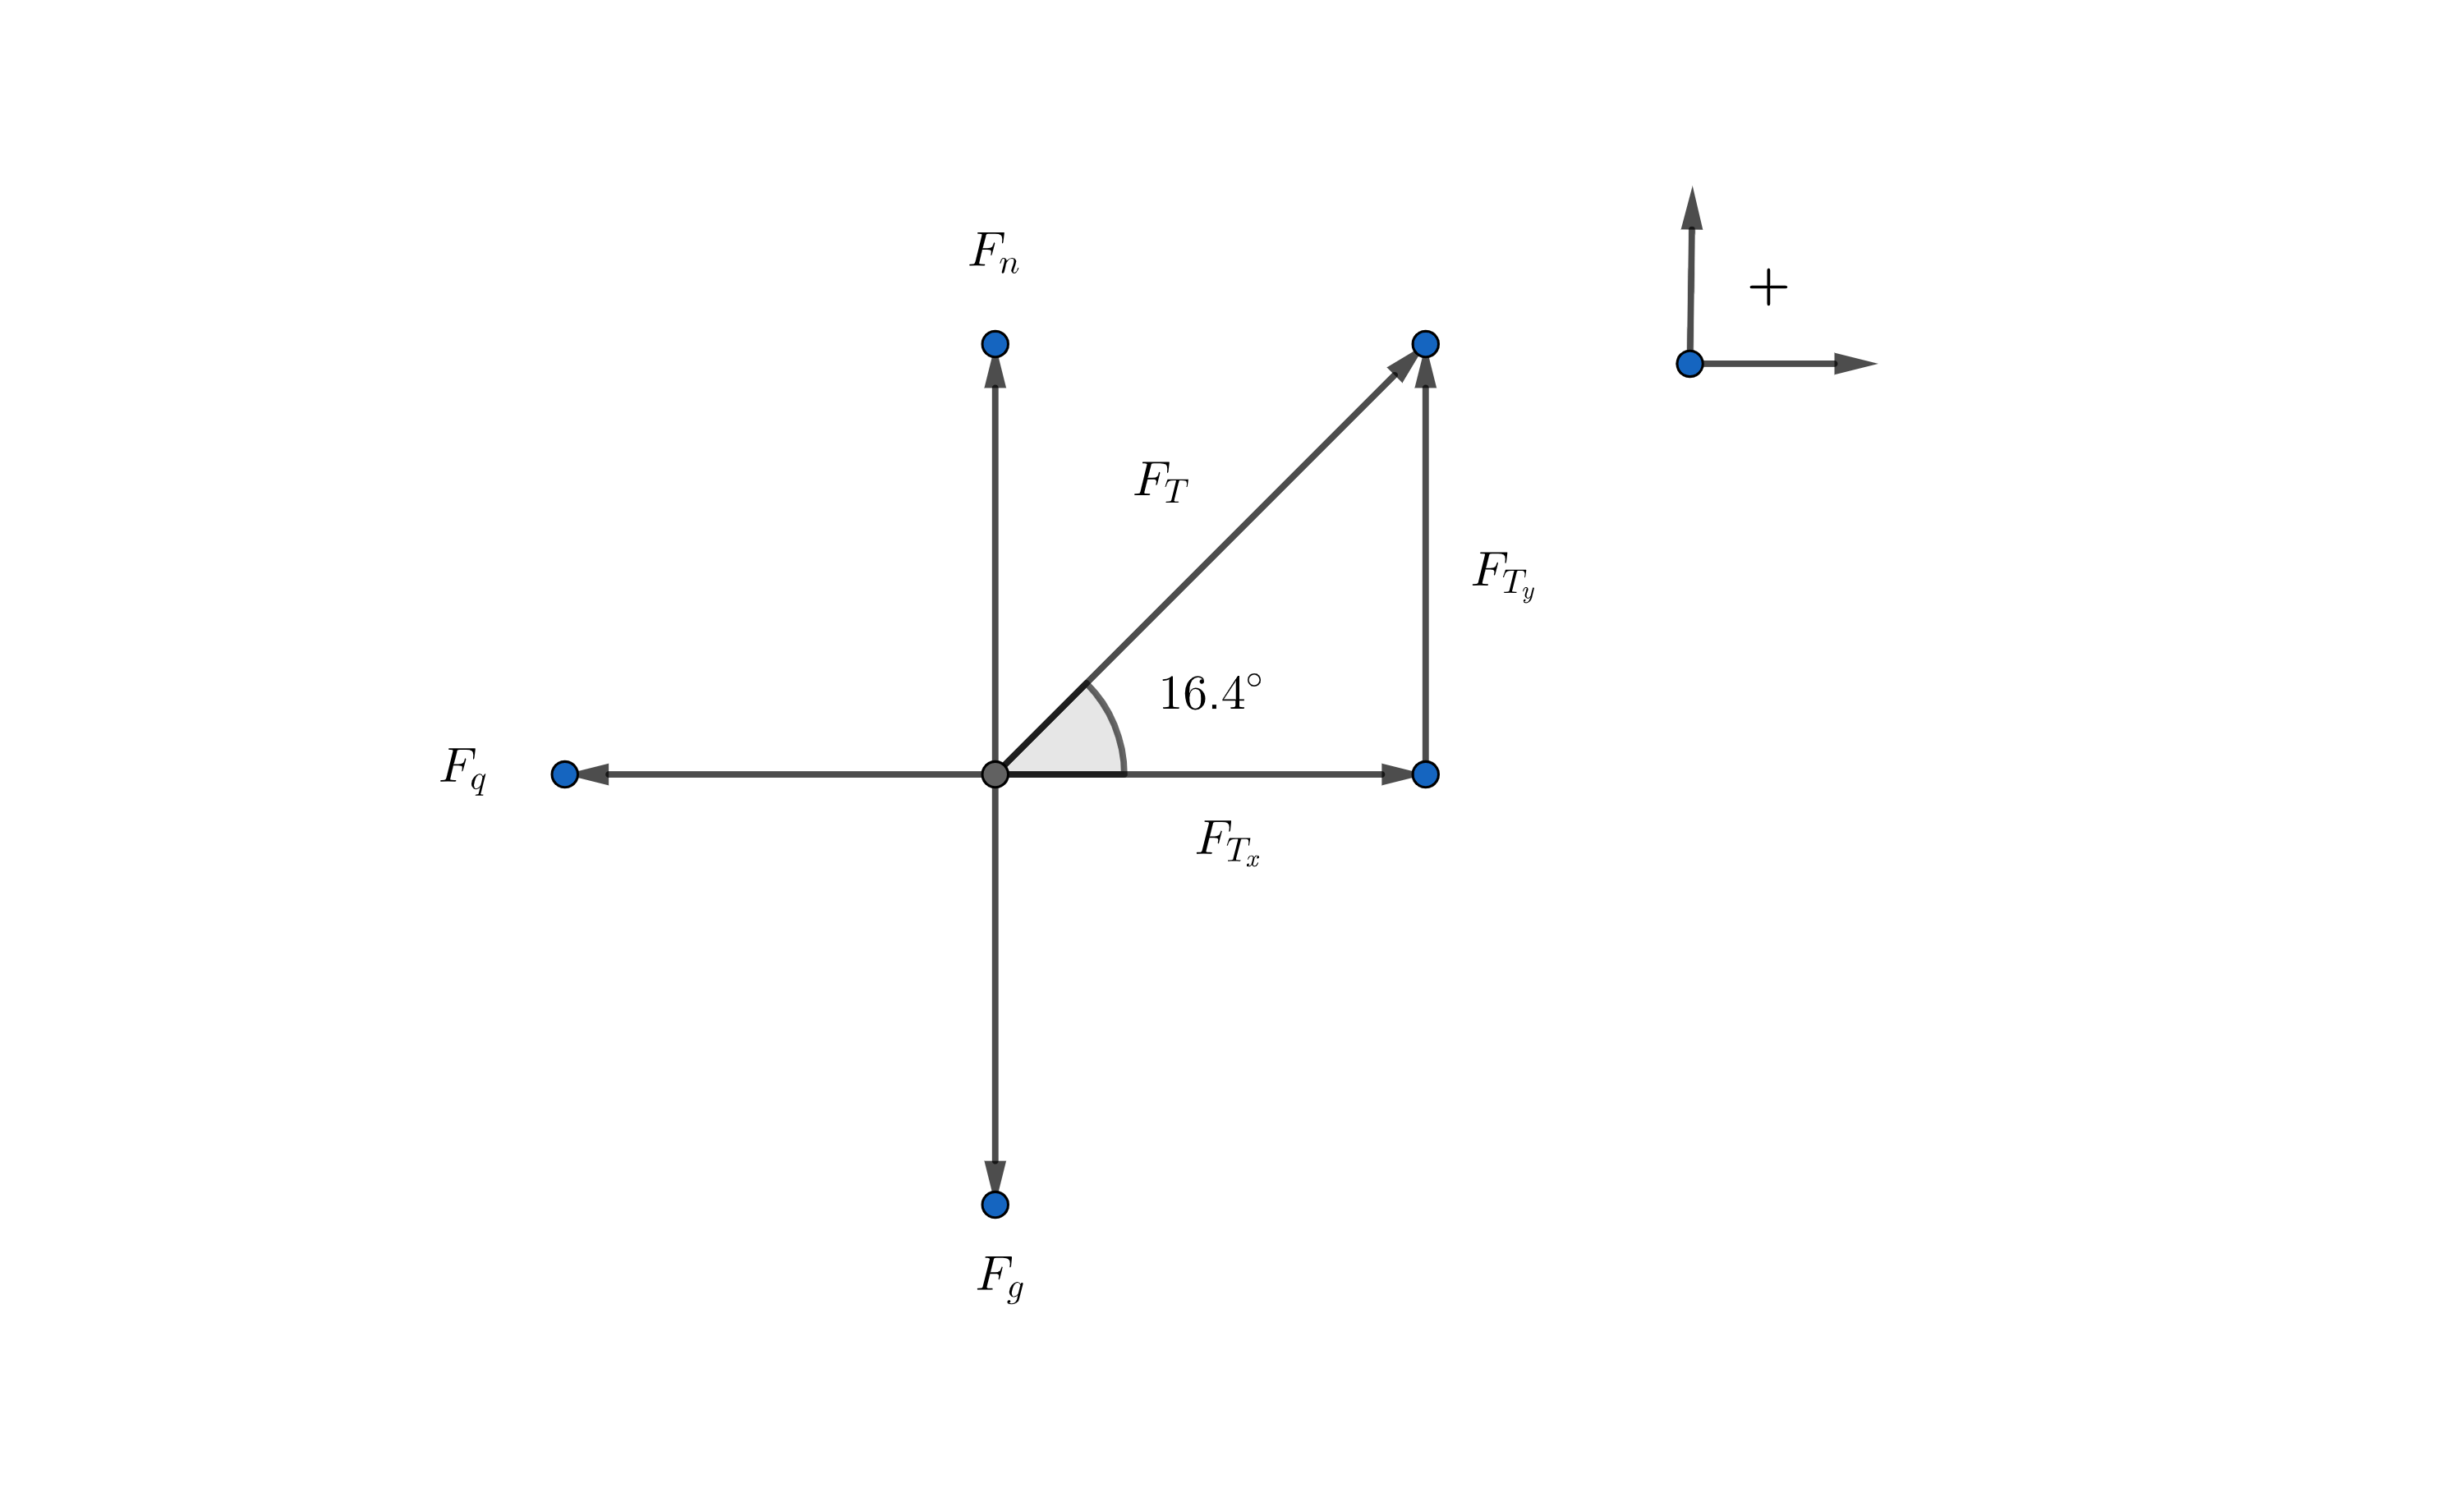
\includegraphics[scale=0.33]{./images/pith_ball_diagram}
\end{minipage}

\vspace*{0.3cm}
\noindent Because we're using the \textbf{\textit{opposite}} and \textbf{\textit{adjacent}} sides of our diagram
($F_{T_{x}}$ and $F_{T_{y}}$) we can rearrange the formula $\tan\theta = \left(\frac{F_{T_{y}}}{F_{T_{x}}}\right)$
to get $F_{T_{x}}$\newline

\noindent\textbf{Final Result:}
\begin{align*}
    F_{q} = F_{T_{x}} & = \frac{F_{T_{y}}}{\tan\theta_{average}}          \\\\
                      & = \frac{m_{ball} \times g}{\tan\theta_{average}}  \\\\
                      & = \frac{(0.177 \times 10^{-4})(9.81)}{\tan(16.4)} \\\\
                      & \approx 0.59 \times 10^{-2}N
\end{align*}

\section*{Sources of Error}
\subsection*{Errors}
\begin{enumerate}
    \item {The force of friction was not accounted for.}
    \item {The ebonite rod was not held directly perpendicular to the pith ball, creating more components.}
    \item {The ebonite rod was not charged similarily to the previous tests.}
\end{enumerate}
\subsection*{Solutions}
\begin{enumerate}
    \item {Use materials that are very low in friction and/or account for friction in calculations.}
    \item {This can be resolved by having something to support the position of the ebonite rod.}
    \item {This can be resolved by using a timer to measure how long to rub the ebonite rod with fur.}
\end{enumerate}\leavevmode

\section*{Conclusion}
This lab efficiently demonstrated how to solve for the electrostatic force of repulsion between a pith ball and an ebonite rod.
By the completion of the lab, it was determined that the electrostatic force of repulsion ($F_{q}$) was approximately $0.59 \times 10^{-2} N$

\section*{Question}
From the data collected during the lab, can you calculate the charge of the pithball? If not, why?\newline

\noindent\textbf{Answer:}
\vspace*{0.2cm}
\begin{adjustwidth}{0.5cm}{0pt}
    Calculating the numerical charge of the pith ball is not possible.
    This is because we don't have enough variables to support the equation:
    $F_{q} = \left(\frac{kq_{a}q_{b}}{{(r_{ab})}^{2}}\right)$
\end{adjustwidth}

\end{document}